% %% %%%%%%%%%%%%%%%%%%%%%%%%%%%%%%%%%%%%%%%%%%%%%%%%%%%%%%%%%%
% intro.tex
%
% Author:  Mauricio Matamoros
% License: MIT
%
% %% %%%%%%%%%%%%%%%%%%%%%%%%%%%%%%%%%%%%%%%%%%%%%%%%%%%%%%%%%%

%!TEX root = ../practica.tex
%!TEX root = ../references.bib

\section{Introducción}%
\label{sec:introduction}
La presente práctica resume los pasos a seguir para leer una señal analógica con un microcontrolador.
En particular, se interesa en la lectura de la temperatura registrada por un sensor LM35 mediante un Arduino UNO/Mega.
Los datos registrados serán posteriormente enviados vía I\textsuperscript{2}C a una Raspberry Pi para llevar una bitácora de temperatura que podrá ser desplegada en un navegador web.

% %% %%%%%%%%%%%%%%%%%%%%%%%%%%%%%%%%%%%%%%%%%%%%%%%%%%%%%%%%%%
% intro-lm35.tex
%
% Author:  Mauricio Matamoros
% License: MIT
%
% %% %%%%%%%%%%%%%%%%%%%%%%%%%%%%%%%%%%%%%%%%%%%%%%%%%%%%%%%%%%


%!TEX ROOT=../main.tex
%!TEX ROOT=../references.bib

% CHKTEX-FILE 1
% CHKTEX-FILE 46

El circuito integrado LM35 es un sensor de temperatura cuya salida de voltaje o respuesta es linealmente proporcional a la temperatura registrada en escala centígrada.
Una de las principales ventajas del LM35 sobre otros sensores lineales calibrados en Kelvin, es que no se requiere restar constantes grandes para obtener la temperatura en grados centígrados.
El rango de este sensor va de \degreesC{-55} a \degreesC{150} con una precisión que varía entre \degreesC{0.5} y \degreesC{1.0} dependiendo la temperatura medida~\Citep{LM35datasheet}.

\begin{figure}
	\centering
	\begin{subfigure}[b]{0.5\columnwidth}
		\centering
		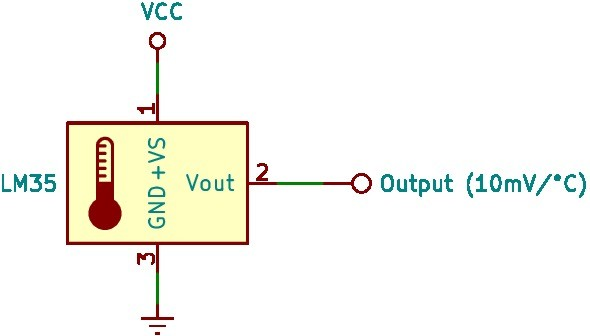
\includegraphics[width=\textwidth,height=5cm,keepaspectratio]{img/lm35a.jpg}
		\caption{Configuración básica: \degreesC{2} a \degreesC{150}}
		\label{fig:lm35config-a} %chktex 24
	\end{subfigure}%
	\begin{subfigure}[b]{0.5\columnwidth}
		\centering
		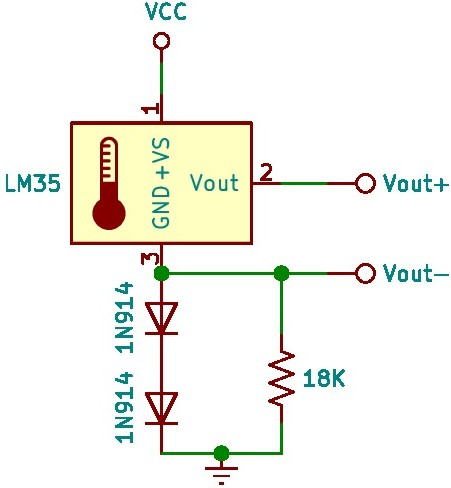
\includegraphics[width=\textwidth,height=5cm,keepaspectratio]{img/lm35b.jpg}
		\caption{Configuración clásica: \degreesC{-55} a \degreesC{150}}
		\label{fig:lm35config-b} %chktex 24
	\end{subfigure}
	\caption{Configuraciones típicas del LM35}
	\label{fig:lm35config} % chktex 24
\end{figure}

Las configuraciones más comunes para este integrado se muestran en la \Cref{fig:lm35config}. La configuración (\Cref{fig:lm35config-a}) básica, la más simple posible pues sólo requiere conectar al integrado LM35 entre \VCC y \GND, permite medir temperaturas entre \degreesC{2} a \degreesC{150}.
Por otro lado, la configuración (\Cref{fig:lm35config-a}) clásica permite medir en todo el rango completo del sensor, es decir entre \degreesC{-55} y \degreesC{150}, pero requiere de un par de diodos 1N914 y una resistencia de 18K$\Omega$ para proporcionar los voltajes de referencia.
En ambos casos, el LM35 ofrece una diferencial de $10mV/^{o}C$, por lo que los voltajes medidos rara vez excederán de 2V respecto a tierra.

Cuando opera en rango completo y las temperaturas registradas son inferiores a cero, se permite un flujo de corriente inverso entre los pines GND y V\textsubscript{out} del LM35, es decir, una salida de voltaje negativo respecto a la referencia.
Debido a que el LM35 no puede generar voltajes inferiores respecto a la referencia del circuito (tierra) se utilizan dos diodos 1N914 en serie colocados en el pin de referencia o tierra del LM35 (véase \Cref{fig:lm35config-b}) para elevar el voltaje del subcircuito del LM35 aproximadamente 1.2V por encima del voltaje de referencia o tierra general.
Así, cuando el LM35 entre en contacto con temperaturas negativas, el voltaje de diodo o V\textsubscript{DD} referenciable mediante la resistencia de 18K hará posible que el voltaje de V\textsubscript{out+} sea inferior al de V\textsubscript{out-} y pueda calcularse la diferencia, tal como se muestra en la~\Cref{tab:lm35}.

\begin{wraptable}{r}{7.0cm}
	\centering
	\caption{Salida de un LM35 en rango completo}%
	\label{tab:lm35} %chktex 24
	\begin{tabular}{rr}%\\
	\toprule
	Temp [\degreesC{}]& V\textsubscript{out+} [V] \\
	\midrule
	-55 & 0.65 \\
	  0 & 1.20 \\
	 50 & 1.70 \\
	100 & 2.20 \\
	150 & 2.70 \\
	\bottomrule
	\end{tabular}
\end{wraptable}
% %% %%%%%%%%%%%%%%%%%%%%%%%%%%%%%%%%%%%%%%%%%%%%%%%%%%%%%%%%%%
% intro-adc.tex
%
% Author:  Mauricio Matamoros
% License: MIT
%
% %% %%%%%%%%%%%%%%%%%%%%%%%%%%%%%%%%%%%%%%%%%%%%%%%%%%%%%%%%%%
% CHKTEX-FILE 1
% CHKTEX-FILE 46
%!TEX root = ../practica.tex
%!TEX root = ../references.bib

\subsection{Convertidor Analógico---Digital}%
\label{sec:intro-adc}
Para leer la señal del LM35 se requiere de un Convertidor Analógico Digital o ADC (por sus siglas en inglés: \emph{Digital-Analog Converter}).
Un ADC se elige con base en dos factores clave: su precisión y su tiempo de muestreo.
Debido a que la aplicación del ADC será convertir mediciones de temperatura y los cambios de temperatura son muy lentos,\footnotemark{} puede obviarse el tiempo de muestreo.
En cuanto a la precisión, los convertidores A/D más comunes son de 8 y 10 bits, de los cuales ha de elegirse uno.

La precisión del ADC se calcula tomando en cuenta el rango de operación y la precisión del componente analógico a discretizar.
El LM35 tiene un rango de \degreesC{205}, una diferencial de voltaje $\Delta{}V=10mV/^{o}C$ y una precisión máxima de \degreesC{0.5}, por lo que el sensor entregará un máximo de 2.5V respecto al voltaje de referencia del mismo, con incrementos de 5mV.
Debido a que 256 valores para un rango de \degreesC{205} en incrementos de \degreesC{0.5} (es decir 410 valores) es claramente insuficiente para este sensor, por lo que será conveniente utilizar un convertidor A/D de 10 bits.

Un ADC típico de 12 bits convertirá las señales analógicas entre voltajes de referencia $V_{Ref-}$ y $V_{Ref+}$ como un entero con valores entre 0 y 4096, interpretando los valores $V_{Ref-}$ como 0 lógico y $V_{Ref+}$ como 4096 de manera aproximadamente lineal.
El decir, la lectura obtenida es directamente proporcional al voltaje dentro del rango, estimable mediante la fórmula:

\begin{equation}
V_{out}= value \times \frac{ V_{Ref+} - V_{Ref-} }{ 4096 }
\end{equation}

En una configuración simple, $V_{Ref-}$ y $V_{Ref+}$ se conectan internamente dentro del RP2040 a tierra y V\textsubscript{CC} respectivamente. Esto simplifica la fórmula como:

\begin{equation}
V_{out}= value \times \frac{ 5V }{ 4096 } = value \times 1.22mV
\end{equation}

En lo concerniente al RP040, éste incorpora un convertidor analógico-digital de 12 bits con soporte para voltaje de referencia $V_{Ref+}$, denominado \emph{ADC\_VREF} según las especificaciones del mismo~\Citep{RP2040datasheet}.
Considerando que el LM35 en rango completo entrega hasta 2.05V ($10mV\times (150 - -55) = 2.05V$) la mayor parte de los 4096 valores jamás serán ocupados.
Por este motivo, conviene sacar partido del pin de voltaje de referencia \emph{ADC\_VREF} del RP2040 mediante un divisor de voltaje (véase~\Cref{fig:lm35-pico}).
En consecuencia, el pin \emph{ADC\_VREF} requerirá de un divisor de voltaje con salida de 2.73V tal como se muestra en la~\Cref{fig:lm35-pico} para dar mayor precisión al convertidor A/D.

\begin{figure}
	\centering
	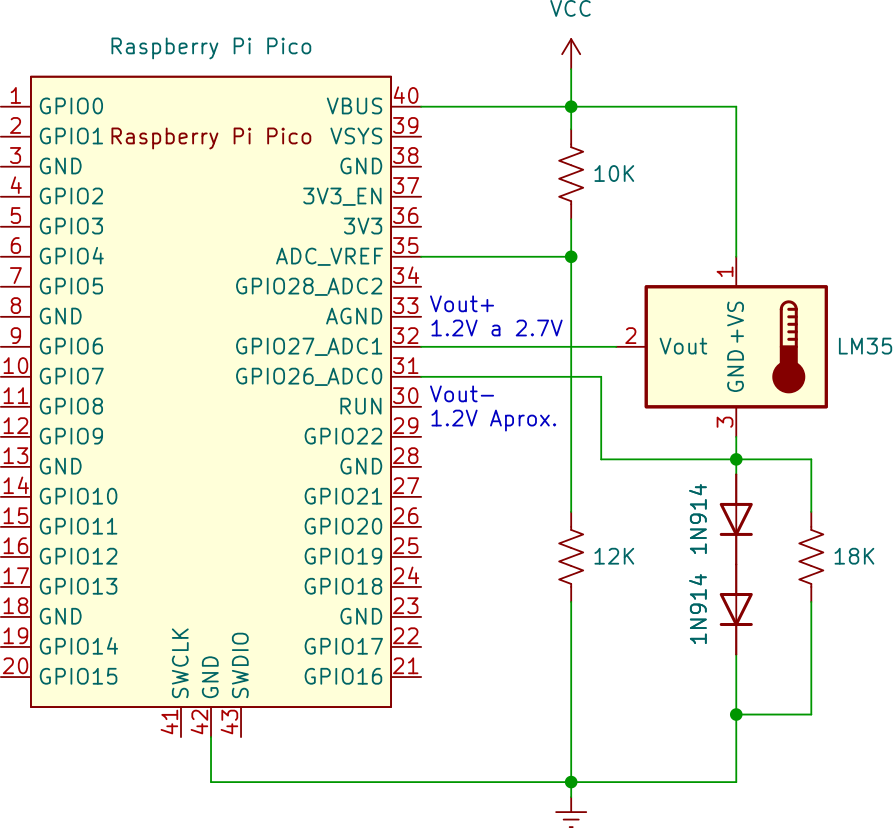
\includegraphics[width=\textwidth,height=7cm,keepaspectratio]{img/lm35-pico.png}
	\caption{Circuito medidor de temperatura LM35 con el RP2040}
	\label{fig:lm35-pico} % chktex 24
\end{figure}

Con esta nueva configuración, se puede calcular de nueva cuenta la precisión del sensor digital una vez decodificado el valor analógico leído del LM35 dividiendo los 2.73V de referencia entre los 4096 valores posibles que entrega el ADC como sigue:

\begin{equation}
\Delta V = \frac{ 2.73V }{ 4096 } =  666.5\times10^{-6}V = 667\mu{}V
\end{equation}

Debido a que la resolución máxima del sensor LM35 determinada por su factor de incertidumbre es de \degreesC{0.5} equivalentes a 0.005V, ambas configuraciones (con y sin el divisor de voltaje) serán adecuadas para operar al sensor.

% %% %%%%%%%%%%%%%%%%%%%%%%%%%%%%%%%%%%%%%%%%%%%%%%%%%%%%%%%%%%
% intro-iic.tex
%
% Author:  Mauricio Matamoros
% License: MIT
%
% %% %%%%%%%%%%%%%%%%%%%%%%%%%%%%%%%%%%%%%%%%%%%%%%%%%%%%%%%%%%

%!TEX root = ../practica.tex
%!TEX root = ../references.bib

\subsection{Bus \IIC}%
\label{sec:intro-i2c}

\begin{wrapfigure}{r}{0.3\columnwidth}
	\centering
	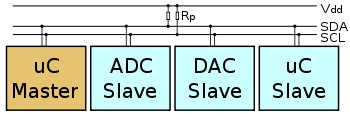
\includegraphics[width=0.3\columnwidth]{img/i2c-bus.png}
	\caption{Bus \IIC}%
	\label{fig:iic-bus}
\end{wrapfigure}
\IIC{} es un protocolo serial inventado por Phillips y diseñado para conectar dispositivos de baja velocidad mediante interfaces de dos hilos (\Cref{fig:iic-bus}).
El protocolo permite un número virtualmente ilimitado de dispositivos interconectados donde más de uno puede ser un dispositivo maestro.
El bus I2C es popular debido a su facilidad de uso y fácil configuración.
Sólo es necesario definir la velocidad máxima del bus, que está conformado por dos cables con resistencias pull-up~\Citep{IICWeb}.

\IIC{} utiliza solamente dos cables: SCL (reloj) y SDA (datos).
La transferencia de datos es serial y transmite paquetes de 8 bits con velocidades de hasta 5MHz.
Además, es requisito que cada dispositivo esclavo tenga una dirección de 7 bits que (el bit más significativo se utiliza para indicar si el paquete es una lectura o una escritura) debe ser única en el bus.
Los dispositivos maestros no necesitan dirección ya que estos generan la señal de reloj y coordinan a los dispositivos esclavos~\Citep{IICWeb}.

